\section{Графы. Способы их представления в памяти компьютера. Матрицы смежости, матрицы инцедентности, списки связности, представление на двух массивах (CSR).}

На протяжении всего билета будем рассматривать граф на иллюстрации ниже

\begin{figure}[h!]
	\centering
	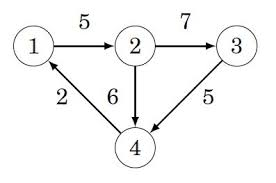
\includegraphics[width=0.4\linewidth]{img_easy/5_1.png}
	\captionsetup{labelformat=empty}
	\caption{На примере этого взвешенного графа в билете мы будем строить разные представдения}
	\label{fig:51}
\end{figure}

\subsection*{Матрицы смежности, матрицы инцидентности, списки связности, представление на двух массивах (CSR).}

\begin{definition}
	\textbf{Графом} называется пара $G=(V, E)$, где $V$ --- множество вершин графа; $E \subset V \times V$ --- множество рёбер графа.
\end{definition}

\subsection{Матрица смежности}
Память: $\Theta(V \times V)$. Элемент на пересечении $i$ строки и $j$ столбца говорит о наличии/отсутствии ребра ($i, j$).

\subsubsection*{Для неориентированного невзвешенного графа:}
$A[i][j]=A[j][i]=1$, если $\exists e=(v_i, v_j)$, иначе $A[i][j]=0$.
А --- симметричная матрица.

\subsubsection*{Для ориентированного невзвешенного графа:}
$A[i][j]=1$, если $\exists e=(v_i, v_j)$, иначе $A[i][j]=0$.
А (в общем случае) несимметричная матрица.

\subsubsection*{Для ориентированного взвешенного графа:}
$A[i][j]=P$, где $P$ --- вес ребра $e=(v_i, v_j)$, если $\exists e=(v_i, v_j)$.
$A[i][j]=C$, иначе, где $C$ --- метка отсутствия ребра, со значением не из диапазона возможных весов.

\subsubsection*{Временные сложности (Матрица смежности):}
\begin{enumerate}
	\item Проверка смежности вершин $x$ и $y$: $O(1)$.
	\item Перечисление всех вершин, смежных с $x$: $O(V)$.
	\item Определение веса ребра $(x, y)$: $O(1)$.
	\item Подсчёт всех рёбер, инцидентных вершине: $O(V)$.
\end{enumerate}

Для графа из примера:
\begin{equation*}
	A = 
	\begin{pmatrix}
		0 & 5 & 0 & 0\\
		0 & 0 & 7 & 6\\
		0 & 0 & 0 & 5\\
		2 & 0 & 0 & 0
	\end{pmatrix}	
\end{equation*}
\subsection{Матрица инцидентности}
Граф задаётся двумерным массивом размера $V \times E$, где каждый элемент $I[i][j]$ говорит о существовании (отсутствии) ребра $e_j$, одним из концов которого является вершина $i$.

\subsubsection*{Для неориентированного невзвешенного графа:}
$I[i][j]=1$, если $e_j=(v_i, v)$ или $(v, v_i)$.
$I[i][j]=0$, иначе.

\subsubsection*{Для ориентированного невзвешенного графа:}
$I[i][j]=1$, если $e_j=(v, v_i)$ (входит в $v_i$).
$I[i][j]=-1$, если $e_j=(v_i, v)$ (исходит из $v_i$).
$I[i][j]=0$, иначе.

\subsubsection*{Для ориентированного взвешенного графа:}
Вместо 1/(-1) храним вес. Можно добавить $+1$-ю строку, где будет храниться вес ребра.

\subsubsection*{Временные сложности (Матрица инцидентности):}
\begin{enumerate}
	\item Поиск $i$-й дуги: $O(V)$.
	\item Подсчёт кол-ва рёбер, инцидентных вершине $x$: $O(E)$.
	\item Для операций с двумя вершинами: $O(V \cdot E)$.
\end{enumerate}

Для графа из примера
\begin{equation*}
	A = 
	\begin{pmatrix}
		-1 & 0 & 0 & 0 & 1\\
		1 & -1 & -1 & 0 & 0\\
		0 & 1 & 0 & -1 & 0\\
		0 & 0 & 1 & 11 & -1\\
		0 & 7 & 6 & 5 & 2
	\end{pmatrix}	
\end{equation*}
где $-1$ --- начало ребра, $1$ --- конец ребра

\subsection{Список смежности}
Массив указателей на списки, где каждой вершине $i$ соответствует указатель на начало списка смежных с $i$ вершин. В элементах этого списка может храниться информация о соответствующем ребре.
Для неориентированных графов элементы списков встречаются в списках обеих вершин. Порядок элементов в списке произвольный.

\subsubsection*{Временные сложности (Список смежности):}
\begin{enumerate}
	\item Проверка смежности вершин: $O(1)$.
	\item Перечисление всех вершин, смежных с $x$: $O(V)$.
	\item Проверка на наличие ребра: $O(1)$.
\end{enumerate}
 Для графа из примера список имеет вид
\begin{equation*}
	\begin{matrix}
	1: &	2\\
	2: & 3 & 4\\
	3: & 4\\
	4: & 	1\\
	\end{matrix}	
\end{equation*}
\subsection{CSR (Compressed Sparse Row)}
Разреженным называется массив, содержащий большое число нулей.
CSR --- способ хранения разреженной матрицы смежности в виде двух (трёх для взвешенных) массивов.

\subsubsection*{Алгоритм:}
У нас есть разреженная матрица смежности.
\begin{enumerate}
	\item Составим массив строчных индексов: будем хранить только индексы, с которых начинается очередная последовательность совпадающих цифр от 0 до $(V-1)$. Получим массив индексов начала информации о вершинах, смежных с той.
	\item Массив `Beca (values)`:
	\begin{verbatim}
		5 7 6 5 2 // веса рёбер
	\end{verbatim}
	\item Массив `Столбцовые индексы (columns)`:
	\begin{verbatim}
		0 1 3 4 // индексация с нуля
	\end{verbatim}
	\item Массив `Строчные индексы (rows)`:
	\begin{verbatim}
		2 3 4 4 1 // рёбра
	\end{verbatim}
\end{enumerate}

\subsubsection*{Итого:}
Граф задаётся 2 (3 для взвешенных) массивами:
\begin{enumerate}
	\item Содержит индексы столбцов, содержащих ненулевые элементы (кол-во рёбер = $E$).
	\item Показывает индексы массива, определяющие начало и конец каждой строки (кол-во вершин = $V$).
	\item Показывает веса ненулевых рёбер (кол-во рёбер = $E$).
\end{enumerate}

\subsubsection*{Оценка памяти:}
$O(V + 2E) = O(V + E)$ памяти.







